\documentclass[11pt]{article}

\usepackage[left=1.25in,top=1.25in,right=1.25in,bottom=1.25in,head=1.25in]{geometry}
\usepackage{amsfonts,amsmath,amssymb,amsthm}
\usepackage{graphicx, hyperref}
\usepackage{float}


\title{Summary and discussion of: ``Confidence Intervals for Random Forests: The Jackknife and the Infinitesimal Jackknife'' \\
%% replace wih paper title 
{\large Journal club report}}
\author{Zhipeng LIANG}
%% replace with your names
\date{}

\begin{document}
\maketitle

\section{Summary}
\subsection{Bagging and Random Forest}
Suppose that we have training examples $Z_1 = (x_1, y_1), ..., Z_n = (x_n, y_n)$, the dataset $\mathcal{D}=\{Z_i\}_{i=1}^n$, an input $x$ to a prediction problem, and a base learner $\hat{\theta} = t(x;Z_1, ..., Z_n)$.

For bagging method, we stabilize the base learner $t$ by resampling the training data. 
The bagging can be viewed as the solution to 
\begin{equation}
	\label{eq:bagging}
	\hat{\theta}^{B}(x)=\frac{1}{B} \sum_{b=1}^{B} t_{b}^{*}(x), \text { where } t_{b}^{*}(x)=t\left(x ; Z_{b 1}^{*}, \ldots, Z_{b n}^{*}\right),
\end{equation}
where the $Z^{*}_{bi}$ are the $i$-th elements in the $b$-th bootstrap sample.

Moreover, the random forest constructs trees base on not only bootstrap samples but also random feature selection.
Thus it can be viewed as the solution to the following problem 
\begin{equation}
	\label{eq:random-forest}
	\hat{\theta}^{R F}(x)=\frac{1}{B} \sum_{b=1}^{B} \frac{1}{K} \sum_{k=1}^{K} t_{b}^{*}\left(x ; \xi_{k b}, Z_{b 1}^{*}, \ldots, Z_{b n}^{*}\right) \text{ with } \xi_{k b} \stackrel{\mathrm{iid}}{\sim} \Xi,
\end{equation}
where $\xi_{kb}$ can be viewed as the modeling for the feature selection noise.


To be specific, we introduce the generalized bagged version of $\hat{\theta}^{\infty}(x)$ is defined as 
\begin{equation}
	\label{eq:bagged-version}
	\hat{\theta}^{\infty}(x)=\mathbb{E}_{Z_i\sim P_{*}, \xi \sim \Xi}\left[t\left(x; \xi, Z_{1}^{*}, \ldots, Z_{n}^{*}\right)\right],
\end{equation}
where $P^{*}$ is the bootstrap distribution and $\Xi$ is the auxiliary noise distribution. 
Then \eqref{eq:bagging} can be viewed as a Monte Carlo approximation to the bootstrap distribution $P^{*}$ with trivial distribution $\Xi$ while random forest is a Monte Carlo approximation to both the bootstrap distribution $P^{*}$ and nontrivial auxiliary noise distribution.

First, to understand the bootstrap distribution, note that the empirical distribution is \begin{align*}
	P_{\delta}(x, y)=\frac{1}{n} \sum_{i=1}^{n} \delta\left(x=x_{i}, y=y_{i}\right),
\end{align*}
where $\delta(\cdot)$ is the Dirac mass centered at $(x_i, y_i)$.
Then the bootstrap distribution is \begin{align*}
	P_{*}(x, y)=\frac{1}{n} \sum_{i=1}^{n} \sum_{k=1}^n k\delta\left(x=x_{i}, y=y_{i}\right) \frac{1}{k!}\exp^{-1}.
\end{align*}
The derivation is from the approximation of the poisson distribution with parameter $\lambda=1$ $\operatorname{Poisson}(1)$ to the multinomial distribution $\operatorname{Multi}(n,\frac{1}{n})$ when $n\rightarrow \infty$ since we use Poisson bootstrap here.


\subsection{IJ and J estimator}
The goal of this paper is to study the sampling variance of bagged learners
\begin{align*}
	V(x) = \operatorname{Var}(\hat{\theta}^{\infty}(x)).
\end{align*}

This paper consider two basic estimates of $V(\cdot)$:
\begin{enumerate}
	\item The Infinitesimal Jackknife estimate \begin{align*}
		\widehat{V}_{I J}^{\infty}=\sum_{i=1}^{n} \operatorname{Cov}_{*}\left[N_{i}^{*}, t^{*}(x)\right]^{2}
	\end{align*}
	where $\operatorname{Cov}_{∗}[N_i^{*}, t_{∗}(x)]$ is the covariance between $t^{*}(x)$ and the number of times $N_i^{*}$ the $i$-th training example appears in a bootstrap sample. This is the direct application of the Theorem 1 in~\cite{efron2012model}.
	\item The Jacknife-after-Bootstrap estimate \begin{align*}
		\widehat{V}_{J}^{\infty}=\frac{n-1}{n} \sum_{i=1}^{n}\left(\bar{t}_{(-i)}^{*}(x)-\bar{t}^{*}(x)\right)^{2}
	\end{align*}
	where  $\bar{t}_{(-i)}^{*}(x)$ is the average of $t^{*}(x)$ over all the bootstrap samples not containing the $i$-th example and $\bar{t}^{*}(x)$ is the mean of all the $t^{*}(x)$.
\end{enumerate}

In practice, we can only ever work with a finite number B of bootstrap replicates. The natural Monte Carlo approximations to the estimators introduced above are
\begin{equation}
\label{eq:VIJ-Monte}
\widehat{V}_{I J}^{B}=\sum_{i=1}^{n} \widehat{\operatorname{Cov}}_{i}^{2} \text { with } \widehat{\operatorname{Cov}}_{i}=\frac{\sum_{b}\left(N_{b i}^{*}-1\right)\left(t_{b}^{*}(x)-\bar{t}^{*}(x)\right)}{B},
\end{equation}
and
\begin{align*}
\widehat{V}_{J}^{B}=\frac{n-1}{n} \sum_{i=1}^{n} \hat{\Delta}_{i}^{2}, 
\end{align*}
where 
\begin{align*}
	\hat{\Delta}_{i}=\hat{\theta}_{(-i)}^{B}(x)-\hat{\theta}^{B}(x)
\end{align*}
and 
\begin{align*}	
\hat{\theta}_{(-i)}^{B}(x)=\frac{\sum_{\left\{b: N_{b i}^{*}=0\right\}} t_{b}^{*}(x)}{\left|\left\{N_{b i}^{*}=0\right\}\right|},
\end{align*}
where $N_{bi}^{*}$ indicates the number of times the $i$-th observation appears in the bootstrap sample b.

However, these finite-B estimates of variance are often badly biased upwards
if the number of bootstrap samples B is too small. 
To correct the bias, we investigate the bias \begin{align*}
	\mathbb{E}_{*}\left[\widehat{V}_{I J}^{B}\right]-\widehat{V}_{I J}^{\infty}=\sum_{i=1}^{n} \operatorname{Var}_{*}\left[C_{i}\right], \text { where } C_{i}=\frac{\sum_{b}\left(N_{b i}^{*}-1\right)\left(t_{b}^{*}-\bar{t}^{*}\right)}{B}.
\end{align*}

They use the approximation \begin{align*}
	\operatorname{Var}_{*}\left[\left(N_{b i}^{*}-1\right)\left(t_{b}^{*}-\bar{t}^{*}\right)\right] \approx \operatorname{Var}_{*}\left[N_{b i}^{*}\right] \operatorname{Var}_{*}\left[t_{b}^{*}\right]
\end{align*}
which holds when $t(x;Z_1^{*},Z_2^{*},\cdots,Z_n^{*})=\frac{1}{n}\sum_{i=1}^nZ_i^{*}$ as the mean estimator and Poisson bootstrap.
To be specific, the approximation error is dominated by the approximated term.

Thus this bias can be approximated as \begin{align*}
	\mathbb{E}_{*}\left[\widehat{V}_{I J}^{B}\right]-\widehat{V}_{I J}^{\infty}\approx \frac{n}{B^{2}} \sum_{b=1}^{B}\left(t_{b}^{*}(x)-\bar{t}^{*}(x)\right)^{2}.
\end{align*}
Thus we have the bias-correction version
\begin{equation}
	\label{eq:bias-correction-IJ}
\widehat{V}_{I J-U}^{B}=\widehat{V}_{I J}^{B}-\frac{n}{B^{2}} \sum_{b=1}^{B}\left(t_{b}^{*}(x)-\bar{t}^{*}(x)\right)^{2}, 
\end{equation}
and 
\begin{equation}
	\label{eq:bias-correction-J}
\widehat{V}_{J-U}^{B}=\widehat{V}_{J}^{B}-(e-1) \frac{n}{B^{2}} \sum_{b=1}^{B}\left(t_{b}^{*}(x)-\bar{t}^{*}(x)\right)^{2}.
\end{equation}
		
\subsection{Upward Bias and Downward Bias}
Suppose that we have data $Z_1, \cdots, Z_n$ drawn independently from a distribution $F$, and compute the estimate $\hat{\theta}^{\infty}$ from the data as in~\ref{eq:bagged-version}.
Then using the ANOVA decomposition \cite{efron1981jackknife} we know
\begin{equation}
	\label{eq:ANOVA}
	\operatorname{Var}_{F}\left[\hat{\theta}^{\infty}\right]=V_{1}+V_{2}+\ldots+V_{n},
\end{equation}
where $V_k$ are all non-negative.

\cite{efron1981jackknife} also show that, under general condition, the Jacknife estimator of variance is biased upward. To be specific, the Jackknife estimator for the $n+1$-th data point has the variance 
\begin{equation}
	\label{eq:JN-variance}
	\mathbb{E}_{F}\left[\widehat{V}_{J}^{\infty}\right]=V_{1}+2 V_{2}+3 V_{3}+\ldots+n V_{n}.
\end{equation}

However, as pointed out by \cite{IJ, efron2012model}, $\hat{V}_{IJ}^{\infty}$ is equivalent to the vaience of a "bootstrap Hájek projection", i.e.,
\begin{equation}
	\label{eq:IJ-varianc-prepare}
	\widehat{V}_{I J}^{\infty} \approx \sum_{i=1}^{n} h_{F}^{2}\left(Z_{i}\right)
\end{equation}
where $h_{F}(Z)=\mathbb{E}_{F}\left[\hat{\theta}^{\infty} \mid Z_{1}=Z\right]-\mathbb{E}_{F}\left[\hat{\theta}^{\infty}
\right]$.
\eqref{eq:IJ-varianc-prepare} suggests that 
\begin{equation}
	\label{eq:IJ-variance}
	\mathbb{E}_{F}\left[\widehat{V}_{I J}^{\infty}\right] \approx V_{1}.
\end{equation}
Compare \eqref{eq:ANOVA}, \eqref{eq:JN-variance} and \eqref{eq:IJ-variance} we can conclude that Jackknife estimator has a upward bias by double the second-order term, triple the third-term and so on while Infinite Jackknife estimator has a downward bias by dropping higher-order terms.
Thus this paper suggests to use the the arithmetic mean of $\widehat{V}_{J}^{\infty}$ and $\widehat{V}_{IJ}^{\infty}$.

\section{Result and Discussion}
\subsection{Empirical Bayes Calibration}
I learnt \href{https://github.com/swager/randomForestCI}{Stefan Wager's randomForestCI} and \href{https://github.com/scikit-learn-contrib/forest-confidence-interval}{sklearn's randomForestCI} and wrote my own code.
All the figures can be reproduced using the code in \href{https://github.com/liangzp/MATH-5472}{this repository}.
Stefan Wager's code is for R while sklearn's is based on python. 
However, neither of them implemented Jacknife-after-Bootstrap estimator.

\subsection{Figure 2}
In the first experiment I testing the performance of my version of the bias-corrected infinitesimal jackknife estimate of variance for bagged predictors, defined in~\ref{eq:bias-correction-IJ}, on the simulation data.
The experiment setup is the same as described in the paper while here I only outline some points.
The data is generaed via $y=f(x)+\epsilon$ where $\epsilon$ is a Gaussian noise and 
\begin{equation}
	f(x)=\left\{
	\begin{aligned}
	&14 \quad 0.45 \le x\le 0.55\\
	&7 \quad 0.35 \le x\le 0.65\\
	&0 \quad 0\le x\le 1.
	\end{aligned}
	\right
	.
\end{equation}
There is a jump of level 7 at four discontinuous points, 0.35, 0.45, 0.55 and 0.65. 
Thus the ideal variance estimator should capture them.
As we can see, Figure~\ref{lab:figeure2_IJ} shows that the infinitesimal jackknife estimator of the bagging predictors does achieve it.
However, in Figure~\ref{lab:figeure2_J} my version of Jacknife-after-Bootstrap estimator although react to the discontinuous points but fail to capture the true variance.

Before we start to present other experiments, note that both in the originl code by Stefan Wager and sklearn's implementation, the bias-corrected infinitesimal jackknife estimate in~\eqref{eq:bias-correction-IJ} is not directly used.
Instead, Wager conducted empirical Bayes calibration for the infinitesimal jackknife estimate using the g-modeling in \cite{efron2014two}.
Without such a empirical Bayes calibration, most of the elements in the  infinitesimal jackknife estimate will be negative in my implementation.
\begin{figure}[htbp]
	\centering
	\begin{minipage}{.5\textwidth}
	\label{lab:figeure2_J}
	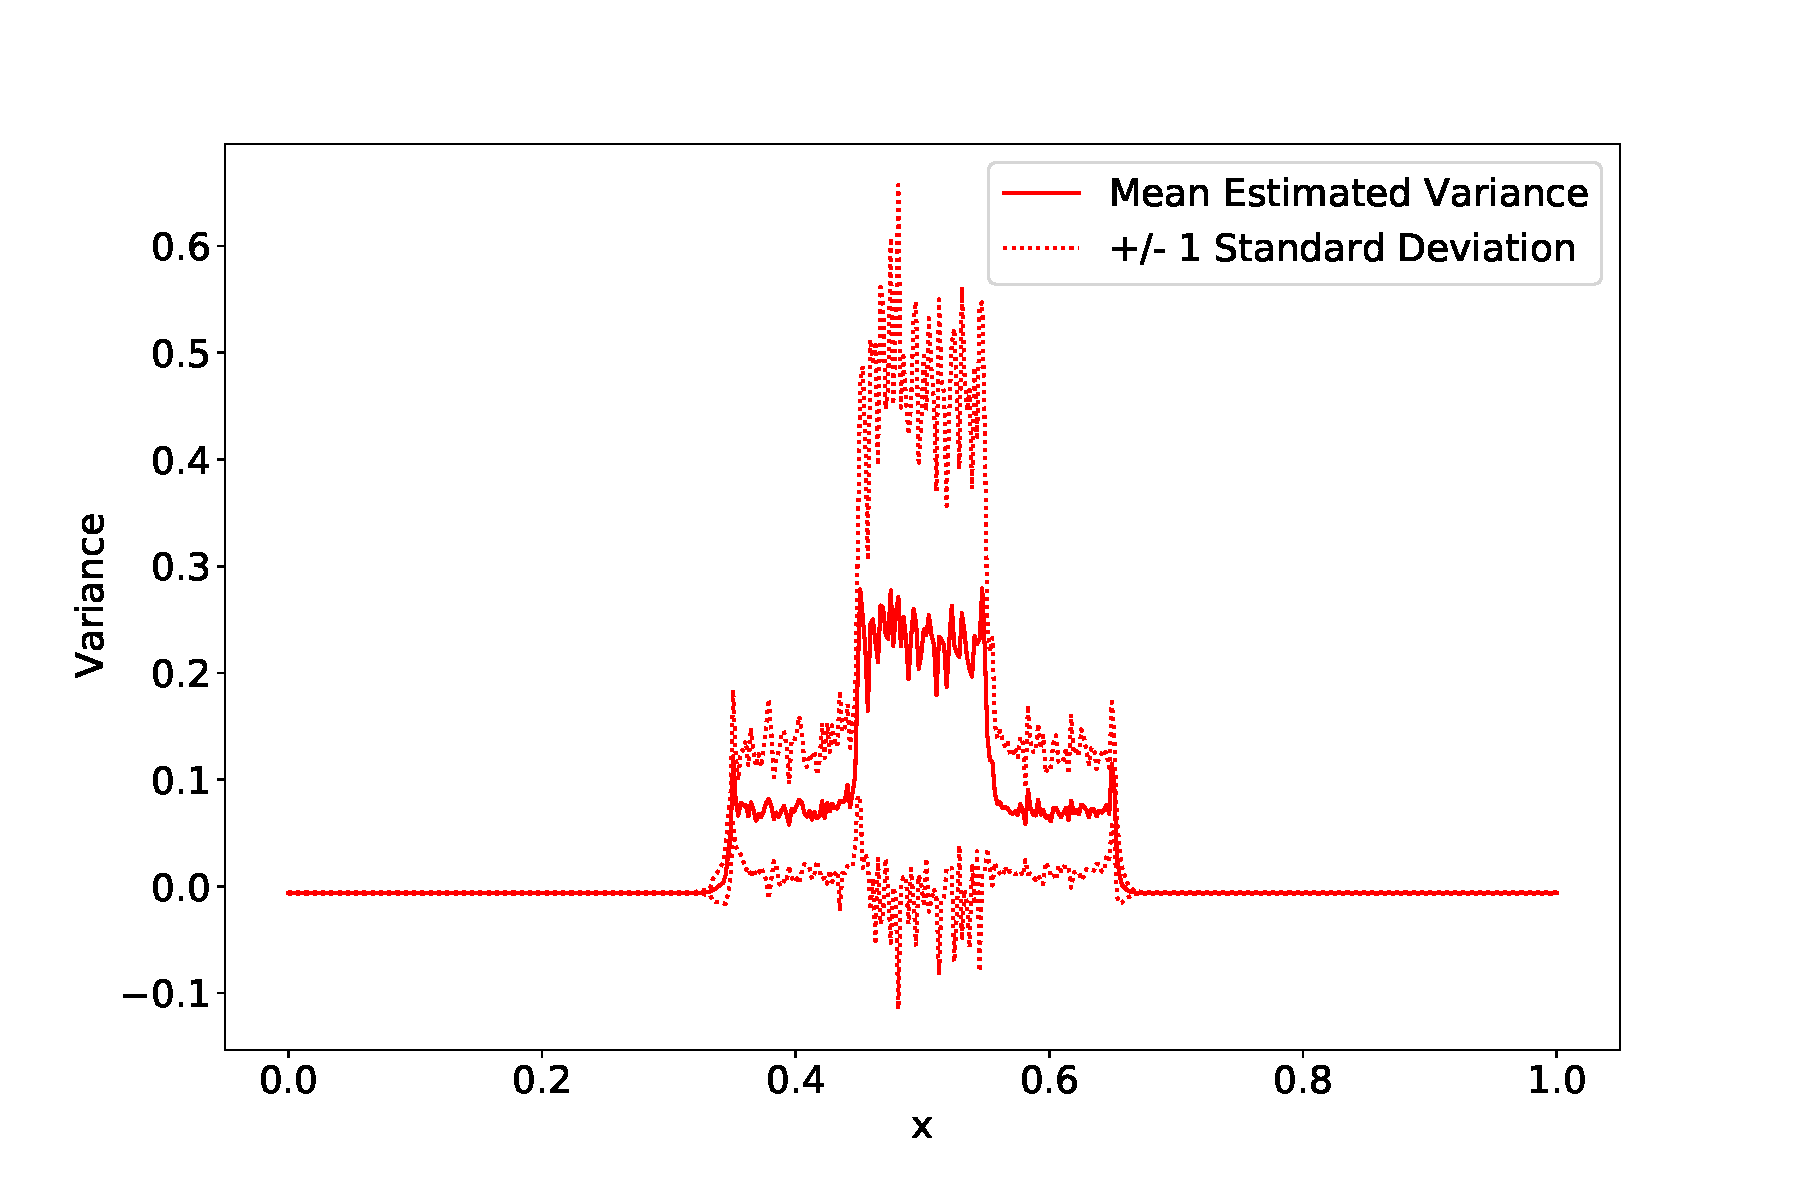
\includegraphics[width=1\textwidth]{../figures/figure2_J.pdf}
	\caption{Jacknife-after-Bootstrap}
	\end{minipage}%
	\begin{minipage}{0.5\textwidth}
	\label{lab:figeure2_IJ}
	\centering	
	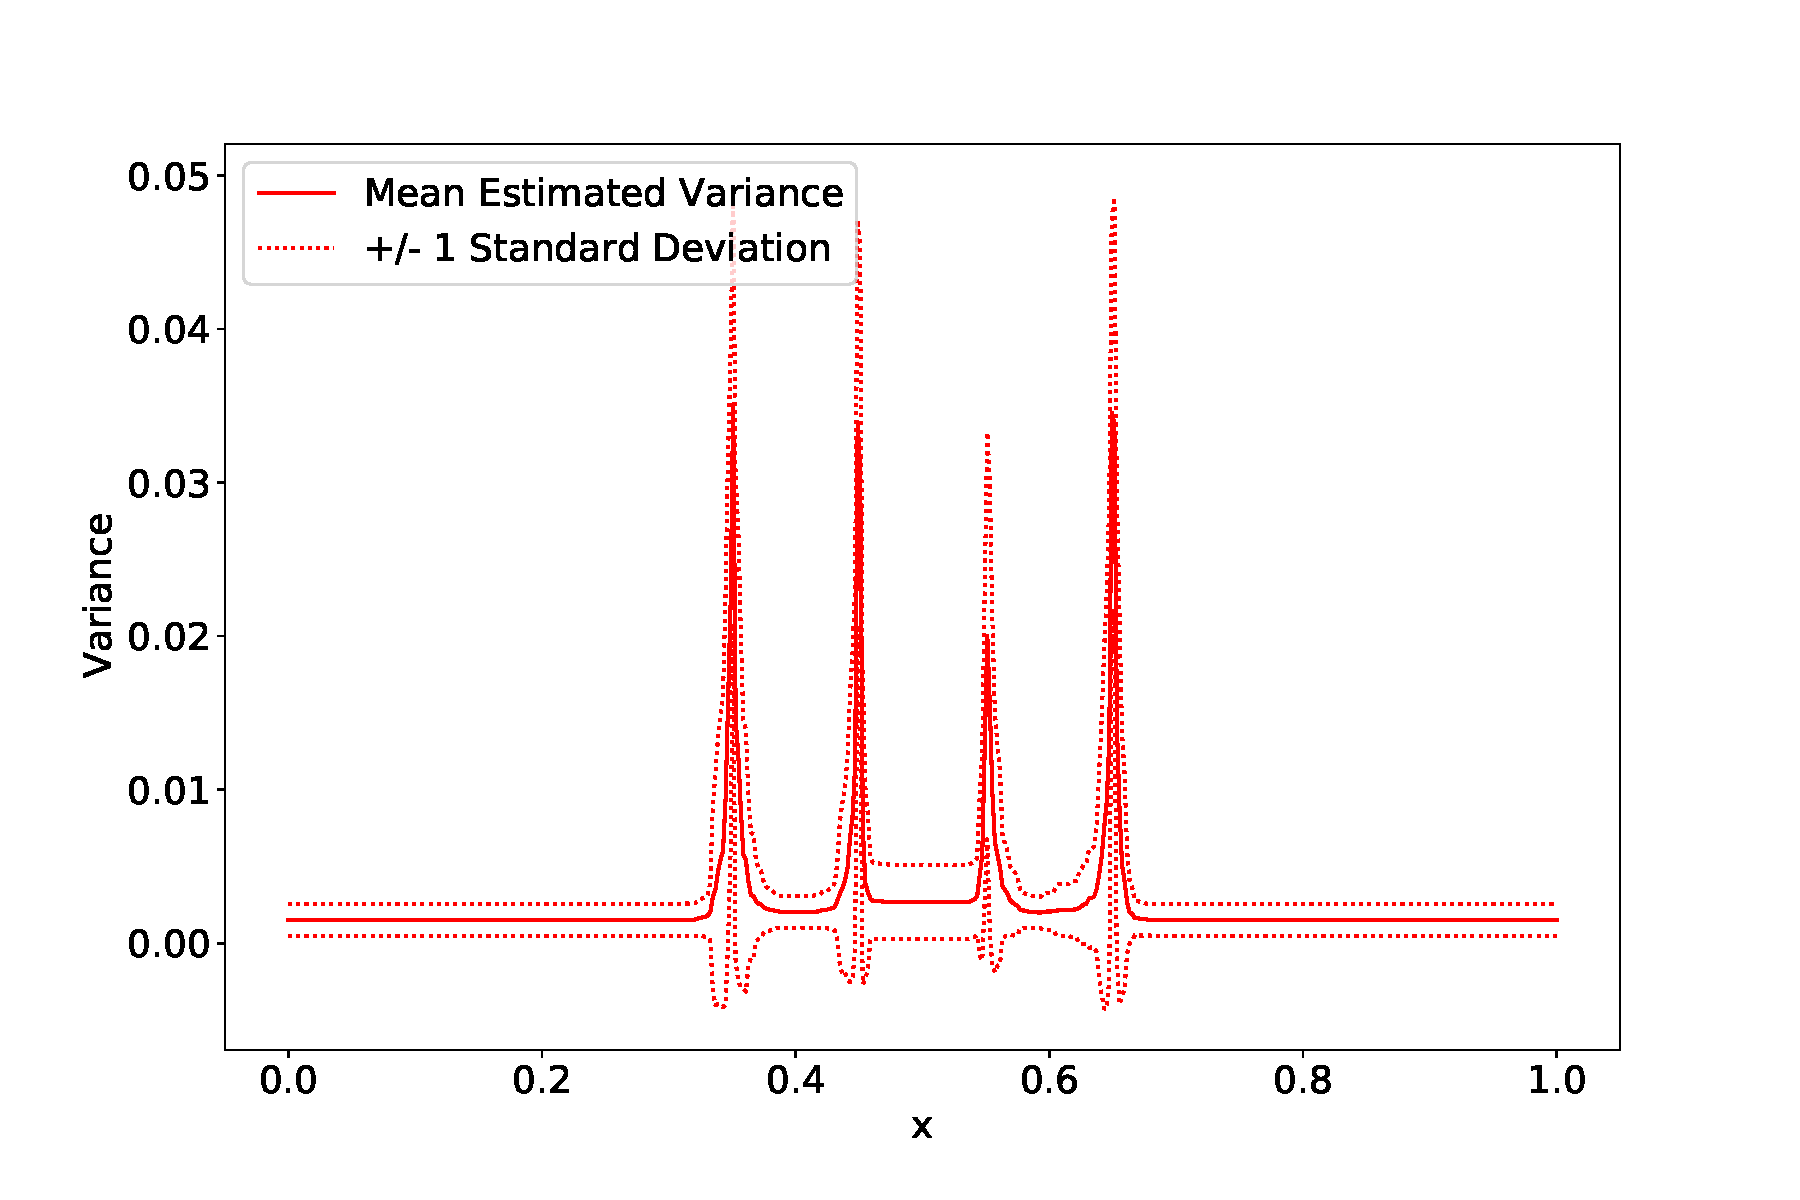
\includegraphics[width=1\textwidth]{../figures/figure2_IJ.pdf}
	\caption{Infinitesimal Jackknife}
	\end{minipage}
\end{figure}

\subsection{Figure 3}
In this experiment, I test the advantage of bias-correction version against.
I test their performance on the cholesterol dataset \cite{efron1991compliance}.
I closely follow the experiment setup in \cite{efron2012model}.
For completeness I outline some key ingredients here.
I use the bagging polyregression and the choice of degree follows $C_p$ criterior \cite{mallows2000some}, i.e., for polyregression regression with degree $m$, the $C_p$ value is defined as
\begin{align*}
	C_{p}(m)=\left\|\boldsymbol{y}-X_{m} \hat{\beta}_{m}\right\|^{2}+2 \sigma^{2} m,
\end{align*}
where $X_m$ is the design matrix with polynomial factors whose degree at most $m$ and 
$$
\hat{\beta}_m = \operatornamewithlimits{argmin}_{\hat{\beta}}\left\|\boldsymbol{y}-X_{m} \hat{\beta}\right\|^{2}.
$$
Follows the setup in \cite{efron2012model}, we use the value $\sigma=22$ in this experiments.
We use the best degree for each bootstrap sample for the final regression model and apply the infinite Jackknife \ref{eq:VIJ-Monte} and bias-correction version \ref{eq:bias-correction-IJ}.
As we can see in Figure~\ref{fig:figure_3}, the bias-correction version (on the right column) is significantly lower than the biased one.
Moreover, as the bootstrap sample sizes increase, the Monte Carlo error decreases which leads to the closer performance between biased IJ and bias-correction one.
\begin{figure}[htbp]
	\label{fig:figure_3}
	\centering
	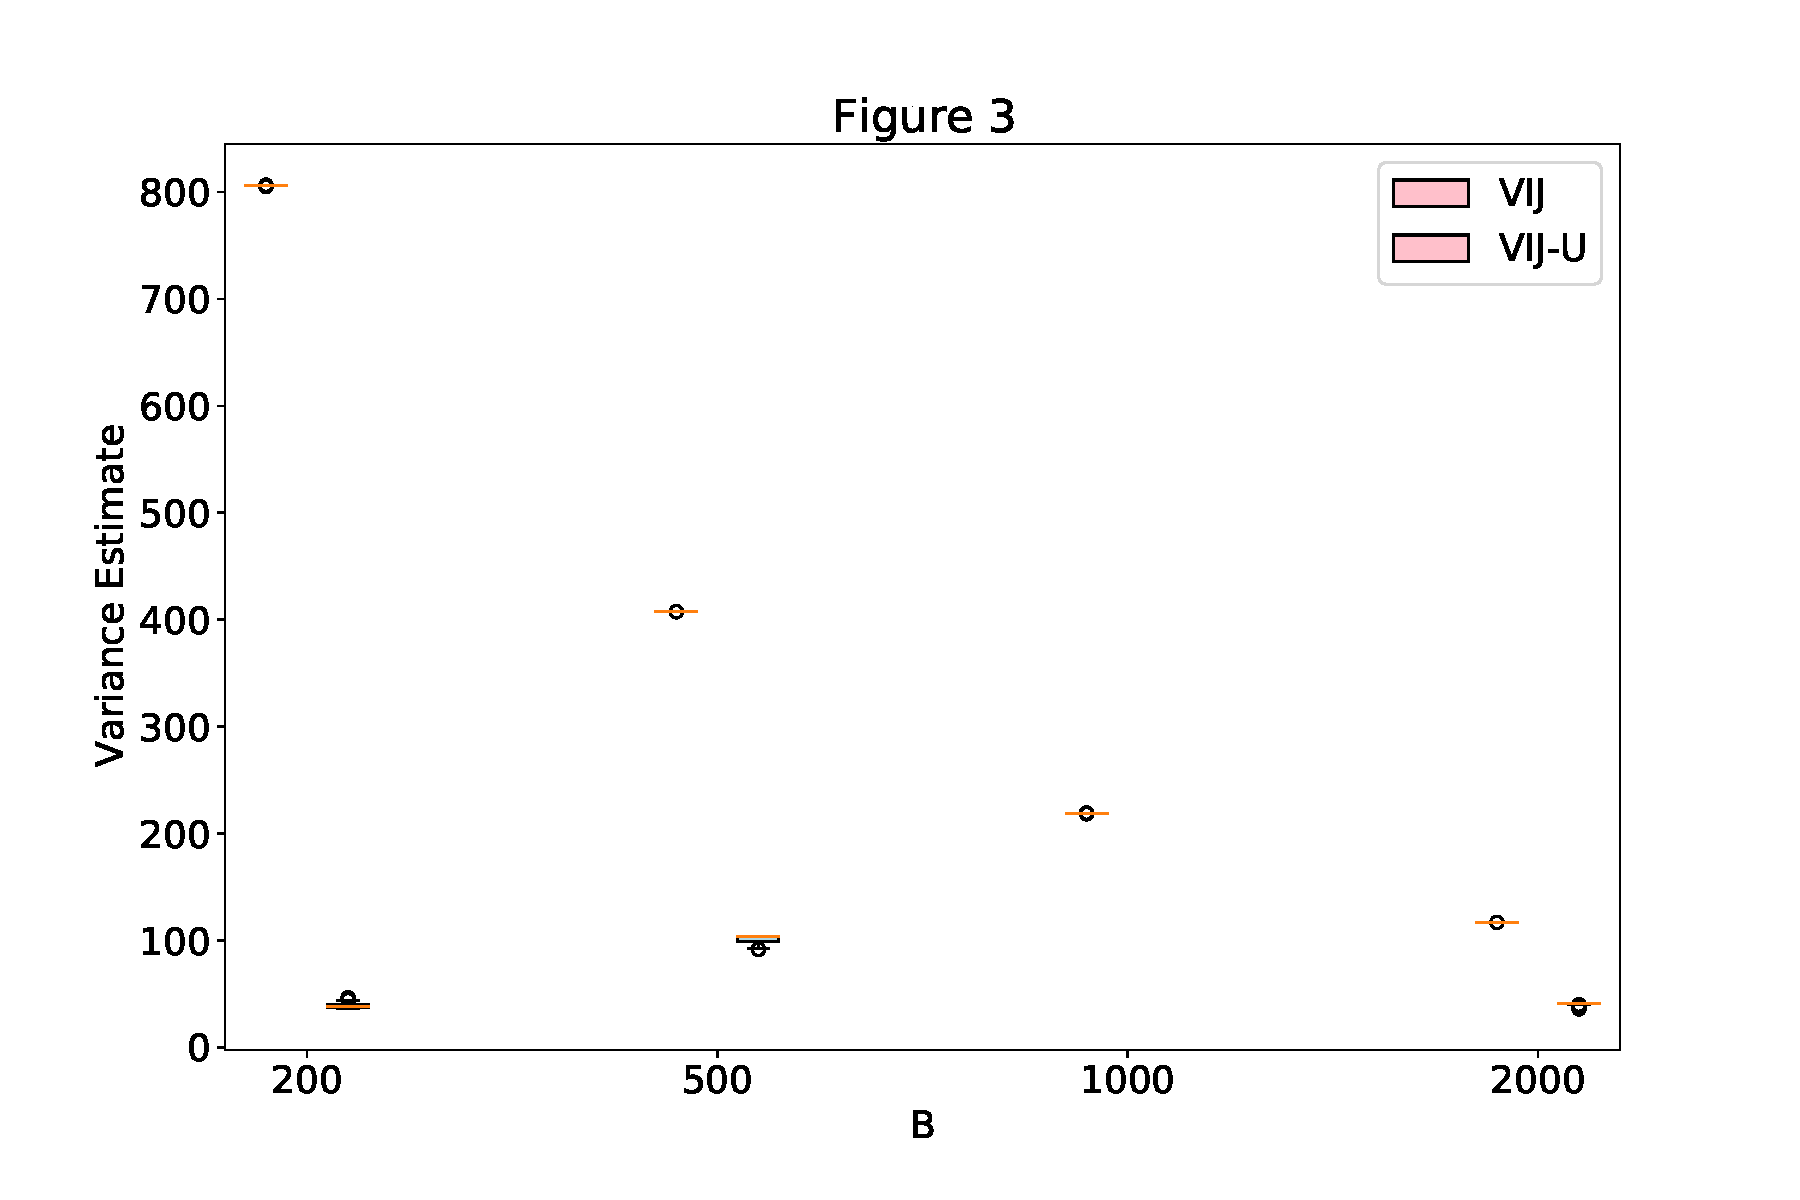
\includegraphics[width=0.8\textwidth]{../figures/figure_3.pdf}
\end{figure}

\subsection{Figure 4}
In this section we aim to gain some qualitative insight from the infinite jackknife estimator on the random forest.
From Figure~\ref{fig:figeure4_1} we plot test-set predictions against IJ-U estimates of standard error for all three random forests with maximum number of features as 5, 19 and 57 (which reduce to the bagging version).
The sample variance increases with the maximum number of select features.
Thus the $m=57$ forest tends to suffer overfitting under this limited sample size, which hinder it from achieving the best test error amongs them.
In contrast, the $m=5$ forest has small variance across all samples, which may implies it suffies from bias due to the limited capacity of utiliziing features.
From Figure~\ref{fig:figeure4_2} we plot the prediction probability of $m=5$ forest versus the difference between prediction probability of $m=19$ against $m=5$.
To visulize the main trend from the scatters, we interpolate the scatters with a polynomial curve with degree 5 (red line).
The red line remains negative when prediction is less than $1/2$ and remains positive when prediction is greater than $1/2$, which implies that the $m=19$ forest has more confidence along the correct direction, and further verify the insight gained from the Infinite Jackknife estimator.
 
\begin{figure}[htbp]
	\centering
	\begin{minipage}{0.6\textwidth}
	\label{lab:figeure4_0}
	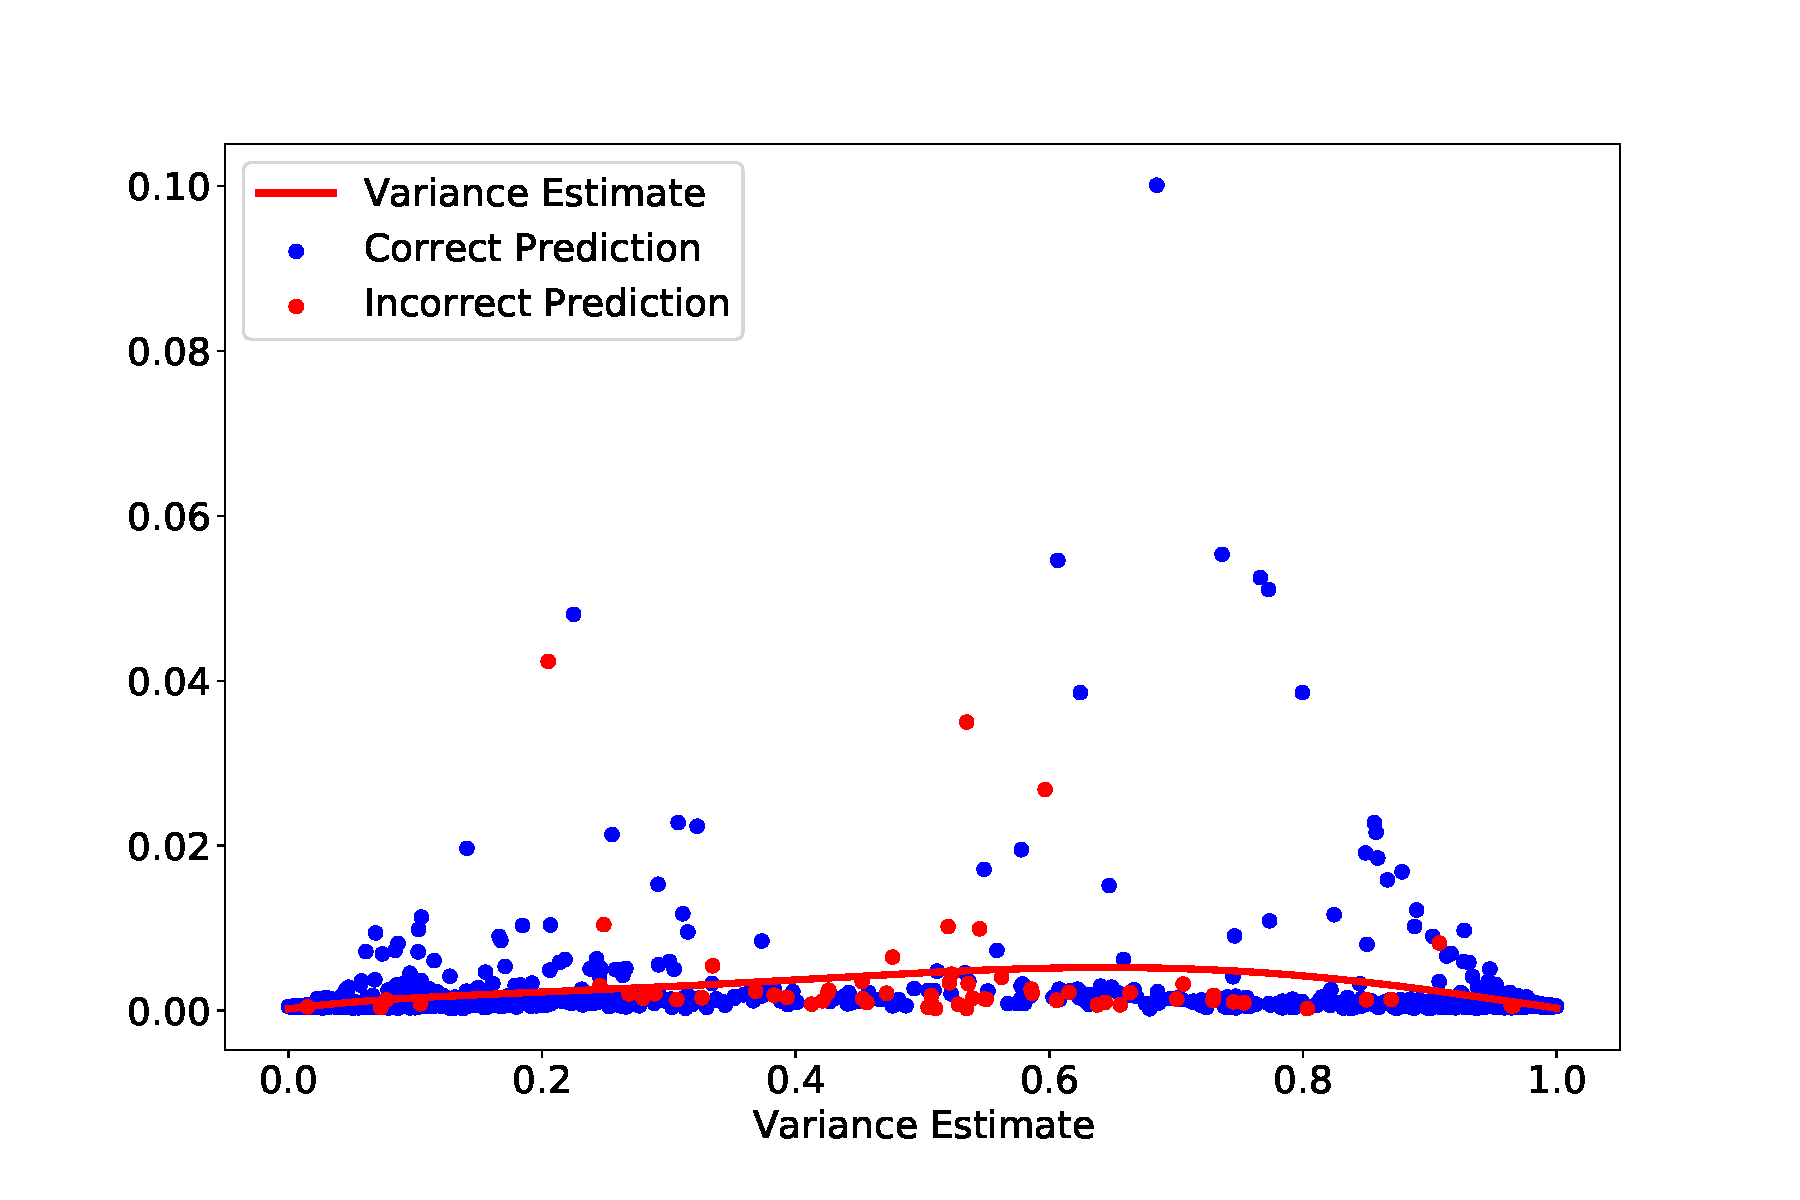
\includegraphics[width=1\textwidth]{../figures/figure4(1)0.pdf}
	\caption{Jacknife-after-Bootstrap}
	\end{minipage}
	\begin{minipage}{0.6\textwidth}
	\label{lab:figeure4_1}
	\centering	
	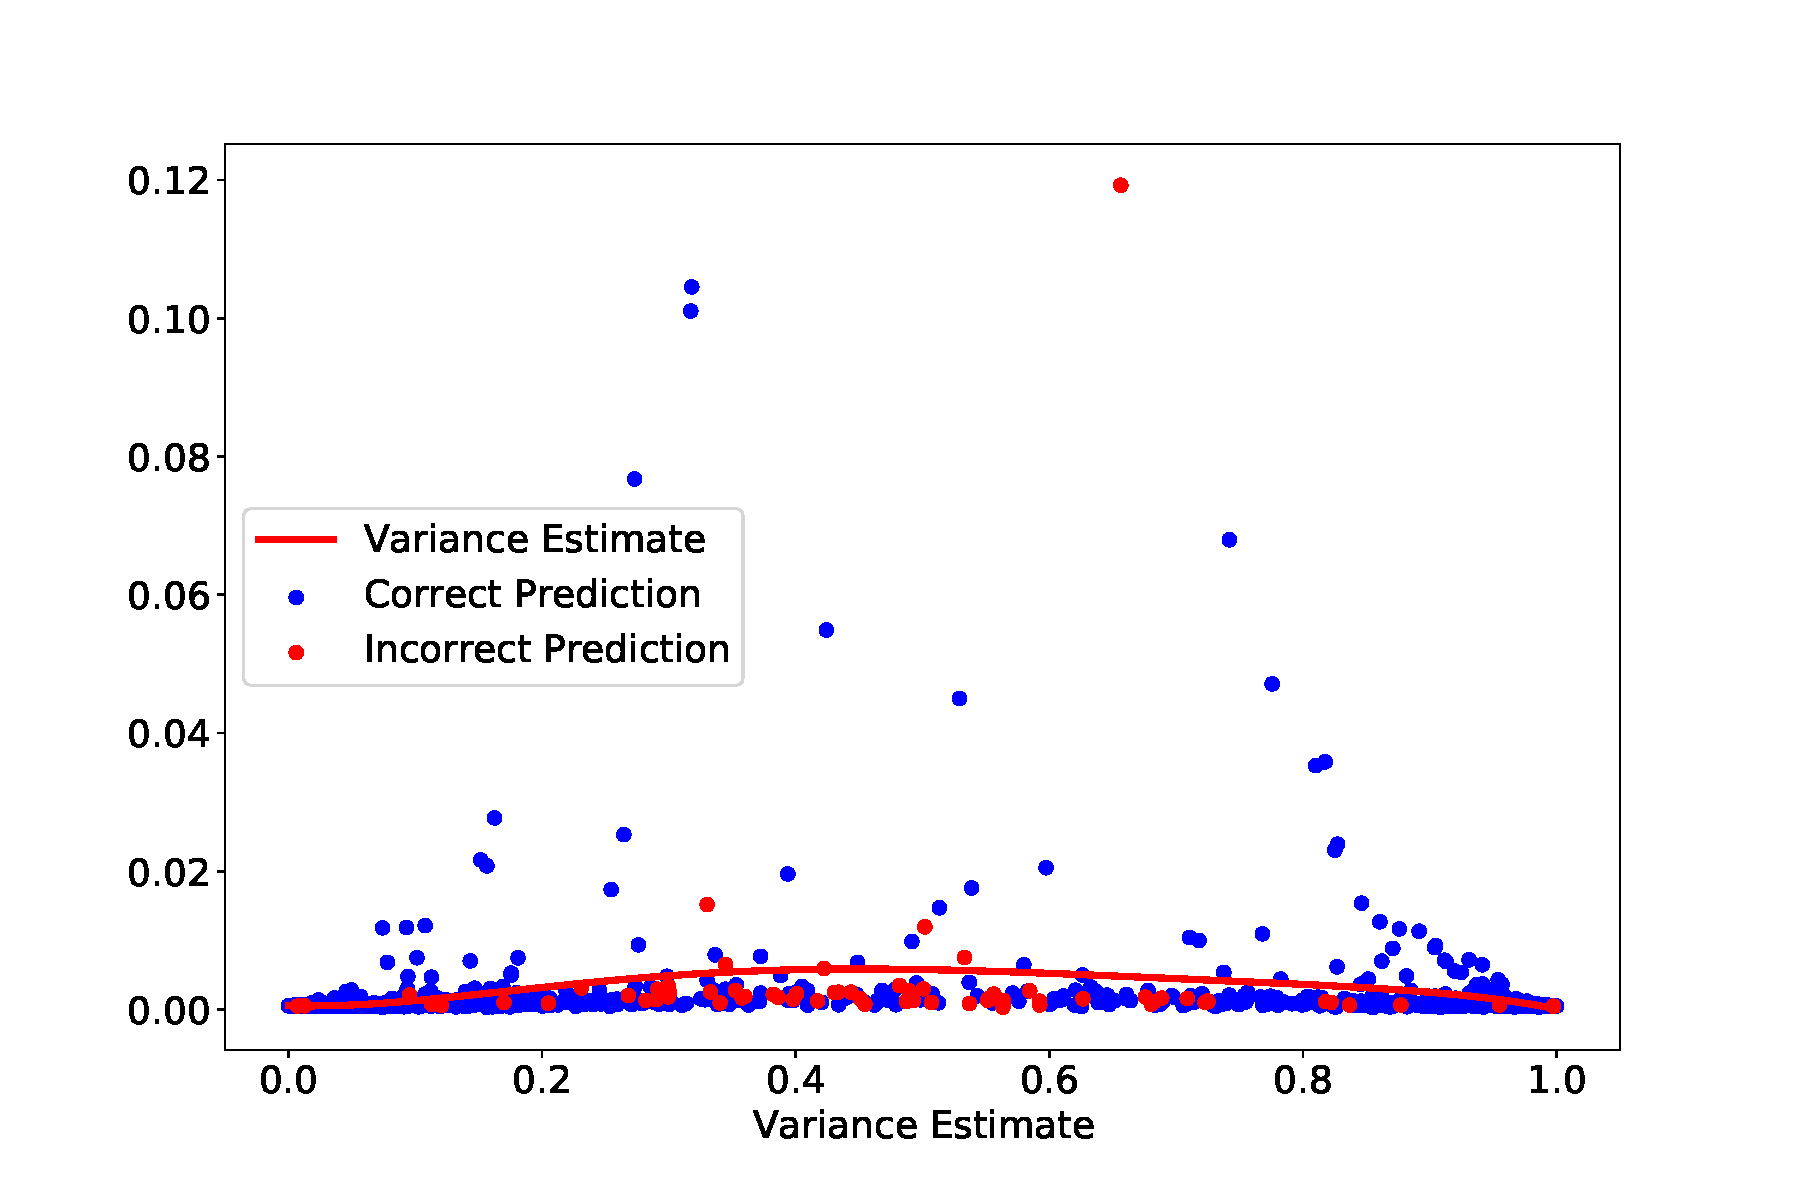
\includegraphics[width=1\textwidth]{../figures/figure4(1)1.pdf}
	\caption{Infinitesimal Jackknife}
	\end{minipage}
	\begin{minipage}{0.6\textwidth}
	\label{lab:figeure4_2}
	\centering	
	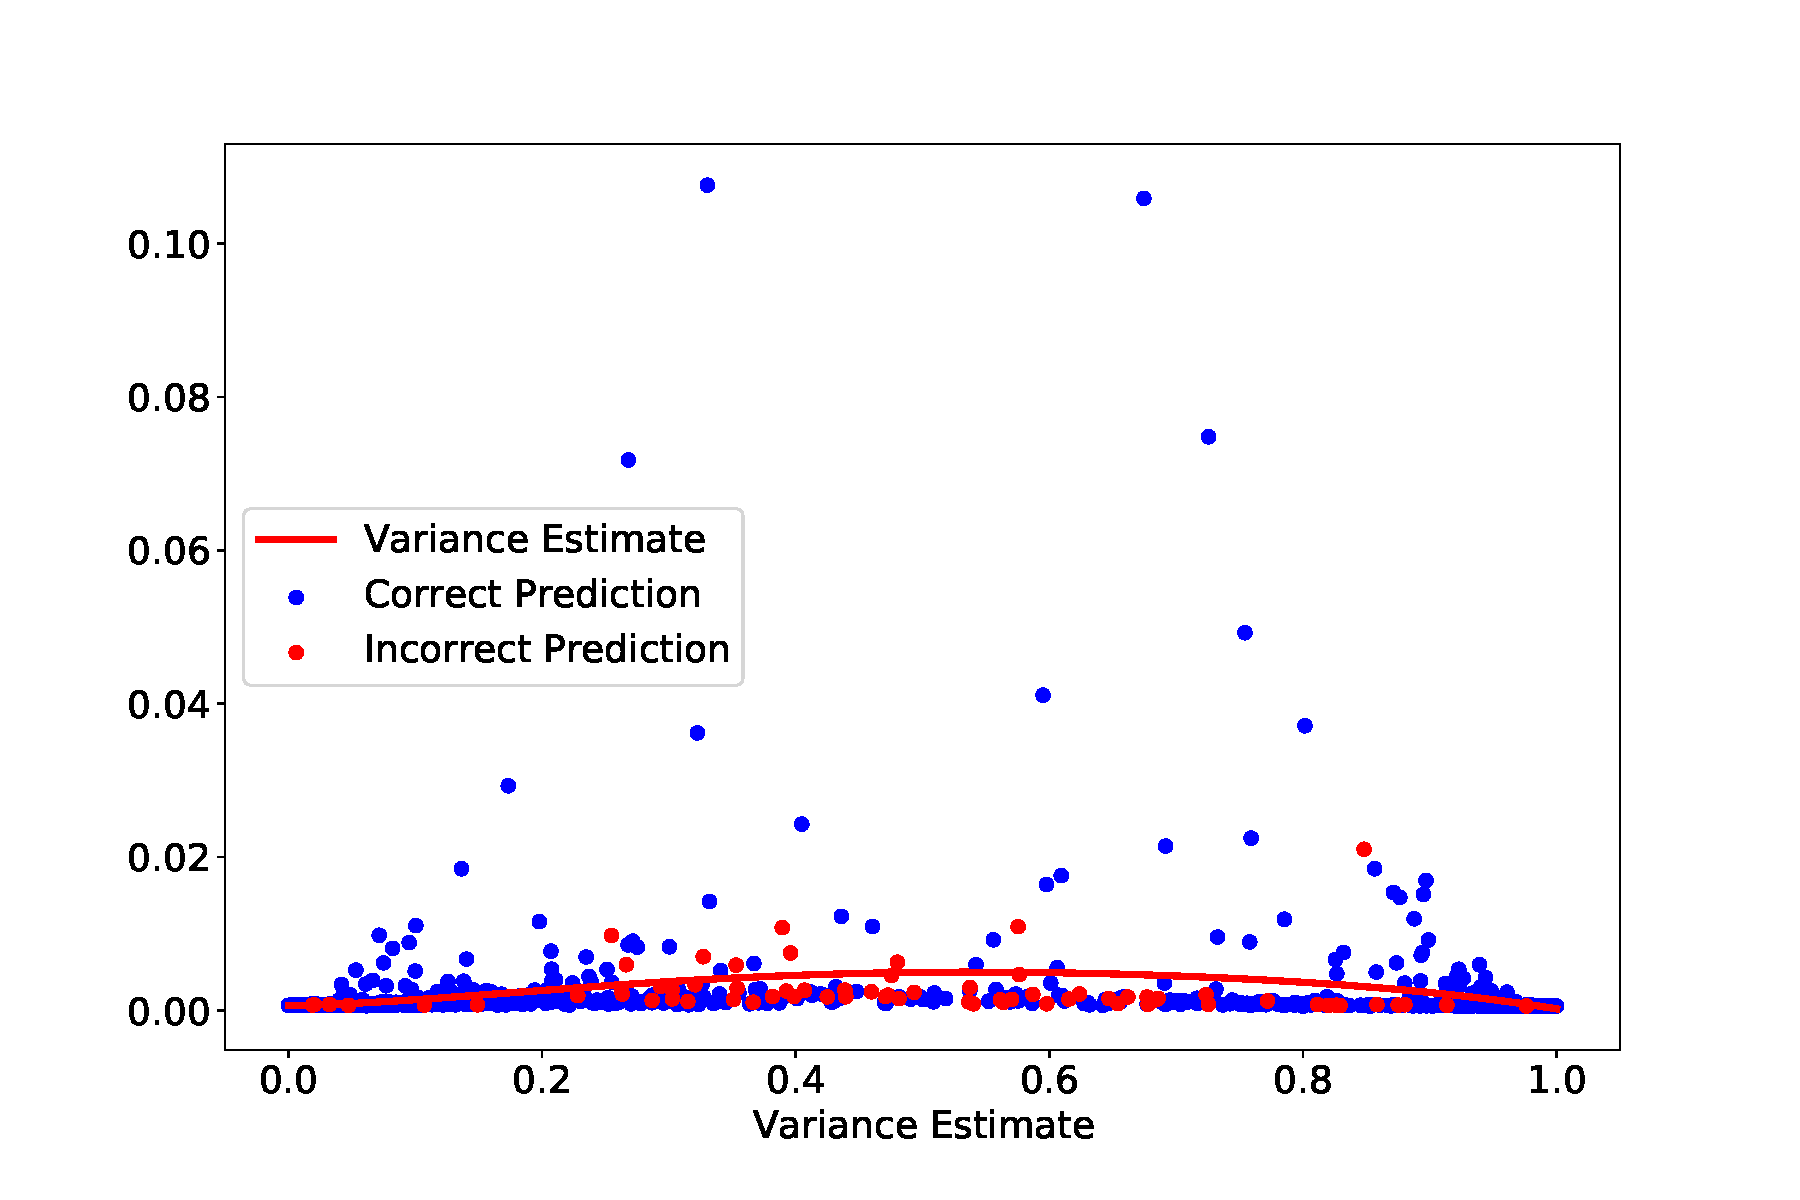
\includegraphics[width=1\textwidth]{../figures/figure4(1)2.pdf}
	\caption{Infinitesimal Jackknife}
	\end{minipage}
\end{figure}

\begin{figure}[htbp]
	\label{fig:figure_4_2}
	\centering
	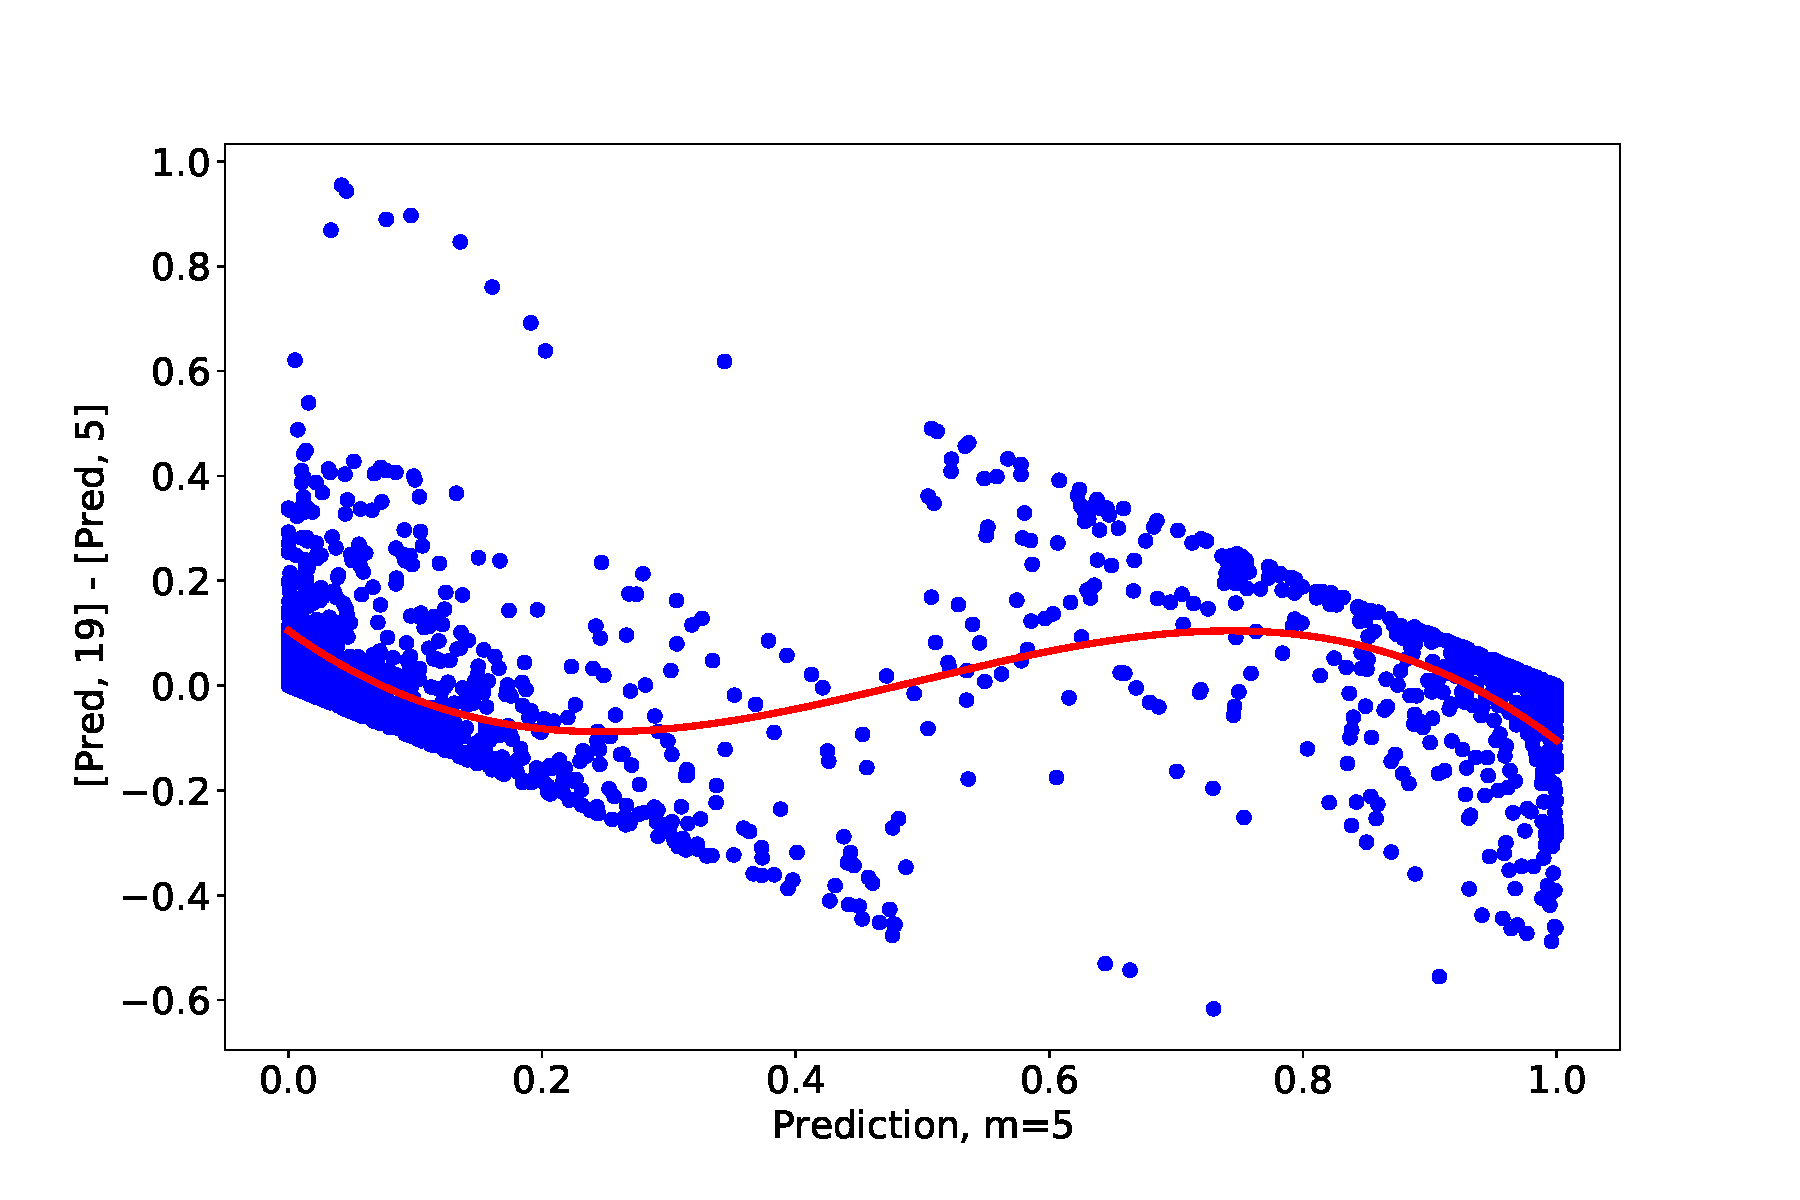
\includegraphics[width=0.8\textwidth]{../figures/figure4(2).pdf}
\end{figure}

\section{Conclusion}

\bibliographystyle{plain} % We choose the "plain" reference style
\bibliography{ref} % Entries are in the refs.bib file
\end{document}